%----------------------------------------------------------------------------------------
%	SOLUTION 3
%----------------------------------------------------------------------------------------
\subsection*{Solution 3.c}
\paragraph{Model 1:}Evolution of accuracy with number of epochs is shown in Fig.~\ref{fig:acc_3c_1}
\begin{figure}[h!]
	\centering
	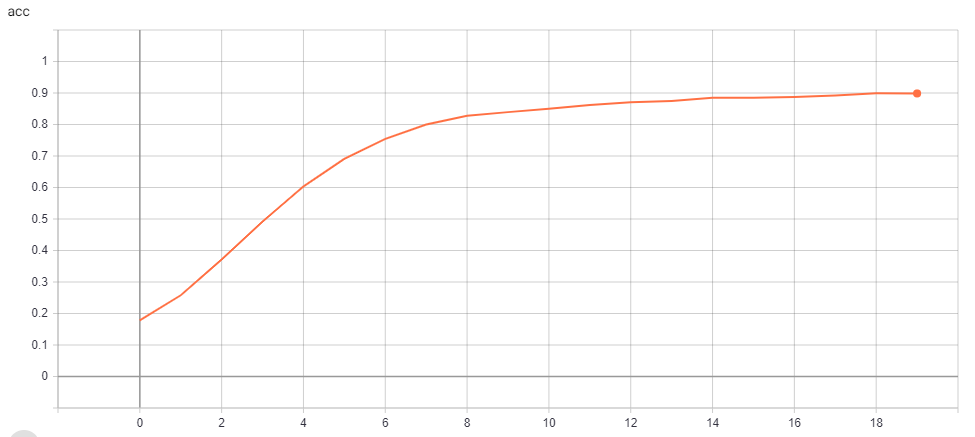
\includegraphics[scale=0.5]{acc_model_1.png}
	\caption{Model 1: Accuracy Vs. Epoch number}
	\label{fig:acc_3c_1}
\end{figure}
 Evolution of loss with number of epochs is shown in Fig.~\ref{fig:loss_3c_1}
\begin{figure}[h!]
	\centering
	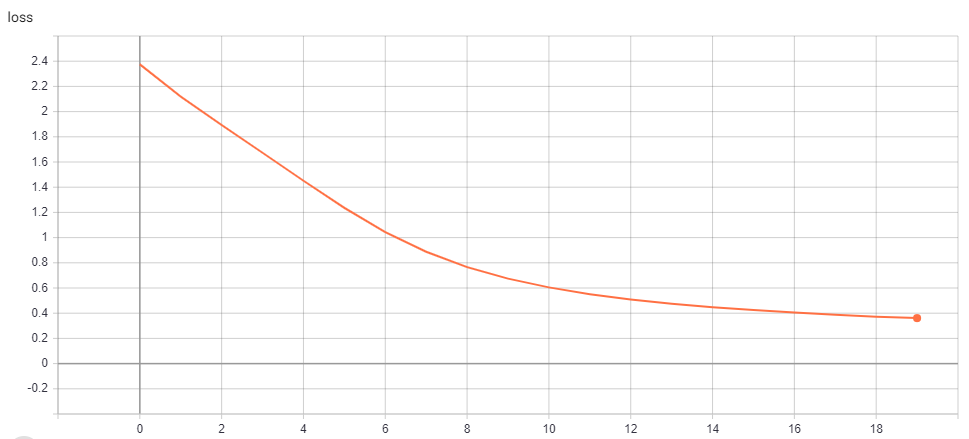
\includegraphics[scale=0.5]{loss_model_1.png}
	\caption{Model 1: Loss Vs. Epoch number}
	\label{fig:loss_3c_1}
\end{figure}
\paragraph{Model 2:}Evolution of accuracy with number of epochs is shown in Fig.~\ref{fig:acc_3c_2}
\begin{figure}[h!]
	\centering
	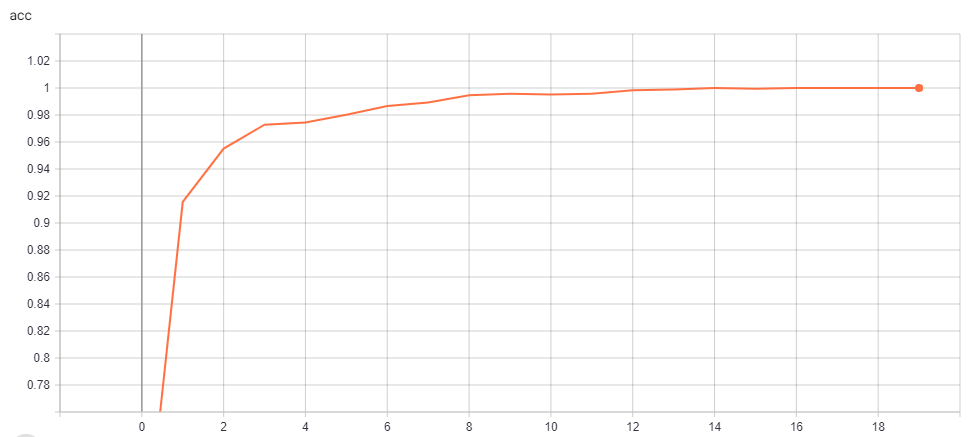
\includegraphics[scale=0.5]{acc_model_2.png}
	\caption{Model 2: Accuracy Vs. Epoch number}
	\label{fig:acc_3c_2}
\end{figure}
Evolution of loss with number of epochs is shown in Fig.~\ref{fig:loss_3c_2}
\begin{figure}[h!]
	\centering
	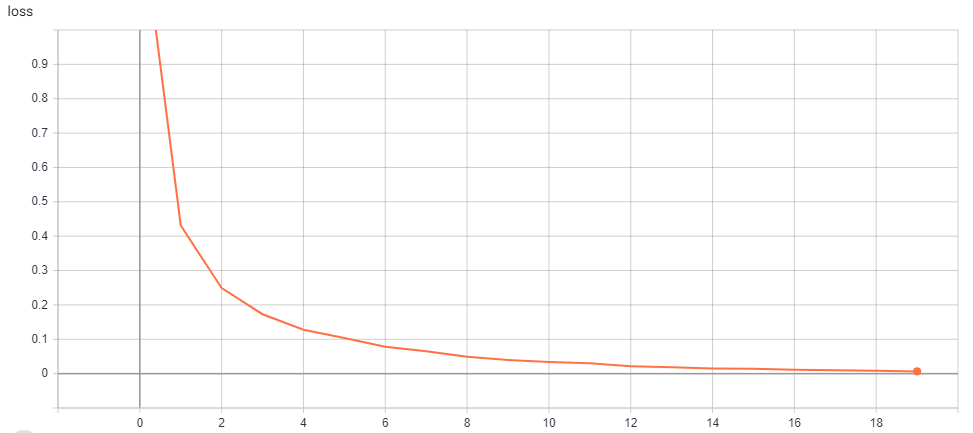
\includegraphics[scale=0.5]{loss_model_2.png}
	\caption{Model 2: Loss Vs. Epoch number}
	\label{fig:loss_3c_2}
\end{figure}
\newpage
Following table captures the accuracy on test data for both the models:
\begin{table}[h!]
	\begin{center}
		\begin{tabular}{||c | c | c ||} 
			\hline
			Model Number & Accuracy(\%) & Log file\\ [0.5ex] 
			\hline\hline
			Model 1 & 89.1 & log\_model\_1\_3c.txt\\ [0.5ex]
			\hline
			Model 2 & 97.5 & log\_model\_2\_3c.txt \\ [1ex]
			\hline
		\end{tabular}
	\end{center}
	\caption{Q3.c: Accuracy on test data}
\end{table}

